\documentclass[12pt,a4paper]{article}
\usepackage[utf8]{inputenc}
\usepackage[spanish]{babel}
\usepackage{amsmath}
\usepackage{amsfonts}
\usepackage{amssymb}
\usepackage[left=2cm,right=2cm,top=2cm,bottom=2cm]{geometry}
\usepackage[T1]{fontenc}
\usepackage{titlesec}
\usepackage{hyperref}
\hypersetup{
    colorlinks=true,
    linkcolor=blue,
    urlcolor=red,
    pdftitle={Tarea 2 set covering},
    }
\author{Lic. Arnoldo Del Toro Peña}
\title{Tarea: Algoritmo Set Covering}
\date{\today}
\usepackage{natbib}
\bibliographystyle{dinat}
\usepackage{graphicx}
\titleformat{\section}[display]
{\normalfont}{\filcenter\small
\ SECCIÓN \thesection   }
{0.5pt}{\Large\bfseries\filcenter  \hrulefill \\ }

%% %--
%\usepackage{titlesec}
%\titleformat{\section}[frame]{\normalfont} %
%{\filright\footnotesize\enspace SECCIÓN \thesection\enspace} %
%{8pt}{\Large\bfseries\filcenter} %
%%-




\begin{document}

\maketitle



\thispagestyle{empty}
\begin{abstract}
    Uso de un método metahurístico para la solución a un problema de set covering utilizando programación en python.
\end{abstract}
{\centering \textit{Palabras clave: python,set, covering, metahurística.}}
\section{Introducción}
En este documento se presentarán los resultados a las instancias obtenidas la siguiente dirección: \href{http://people.brunel.ac.uk/~mastjjb/jeb/orlib/files/}{people.brunel.ac.uk}, se compararán con los resultados óptimos que se presentan a continuación:
\begin{table}[h!]
\centering
\begin{tabular}{|c|c|l|l|l|}
\hline
\multicolumn{1}{|l|}{\textbf{Instancias de Prueba}} & \multicolumn{1}{l|}{\textit{Nombre de la instancia}} & \multicolumn{1}{c|}{\textit{m}} & \multicolumn{1}{c|}{\textit{n}} & \textit{Óptimo} \\ \hline
\textit{4}                                          & scp41                                                & 200                             & 1000                            & 429             \\ \hline
\textit{5}                                          & scp51                                                & 200                             & 2000                            & 253             \\ \hline
\textit{6}                                          & scp61                                                & 200                             & 1000                            & 138             \\ \hline
\textit{A}                                          & scpa1                                                & 300                             & 3000                            & 253             \\ \hline
\textit{B}                                          & scpb1                                                & 400                             & 3000                            & 69              \\ \hline
\textit{C}                                          & scpc1                                                & 400                             & 4000                            & 227             \\ \hline
\textit{D}                                          & scpd1                                                & 400                             & 4000                            & 60              \\ \hline
\textit{E}                                          & scpe1                                                & 50                              & 500                             & 5               \\ \hline
\end{tabular}
\end{table}

Más adelante analizaremos las diferencias entre estos resultados y los que obtuvimos.
\newpage
\section{Descripción}
 El algoritmo que se utilizó fue modificado, la causa de ello es que uno de los archivos a trabajar (scpe1) tenía un conjunto de costos con la cualidad de que todos tenían valor unitario, lo cual en el algoritmo anterior lo que estaba haciendo era seleccionar de manera casi aleatoria cualquier centro, claro esta que no era lo deseado.

\section{Descripción del algoritmo}
 Las modificaciones que se hicieron fueron las siguientes:
 
 \begin{figure}[hbtp]
 \centering
 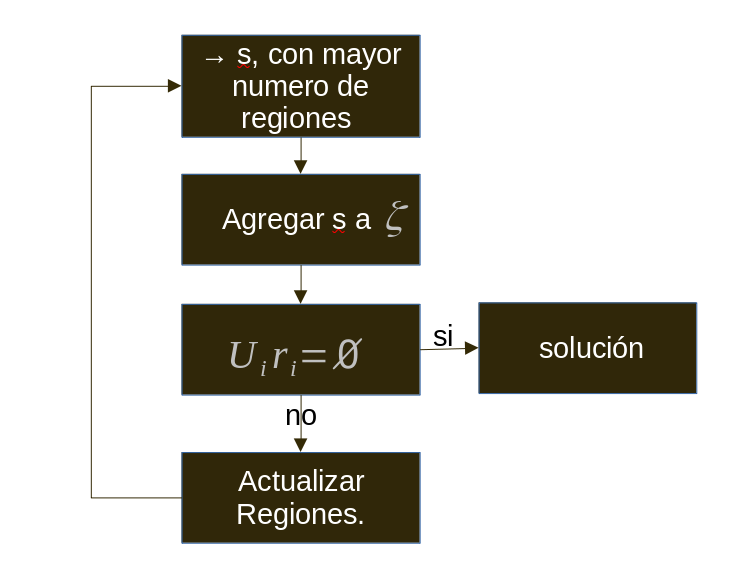
\includegraphics[scale=0.3]{algoritmo set covering.png} \label{algoritmo}
 \caption{Algoritmo corregido}

 \end{figure}
 
 Lo primero que hay que señalar en la figura 1 es que ahora en primera instancia eligiremos al centro que cubra el mayor número de regiones, en segundo lugar agregaremos este centro a nuestro conjunto solución, tomaremos la decisión de avanzar o finalizar dependiendo si hemos cubierto todas las regiones, ya por último repetiremos esto hasta que terminemos de cubrir todas las regiones 
 \newpage
\section{Implementación} 
El algoritmo se programó en lenguaje python con referencias en \cite{van1991guia}, \cite{van2017tutorial} y \cite{chun2001core}, y se puede verificar en el siguiente repositorio de: \href{https://github.com/arnoldae9/PycharmProjects.git}{git-hub}.

\section{Resultados} 
Los resultados se pueden ver en el mismo enlace de git-hub, en los documentos txt, sin embargo se presentarán a continuación en una forma más ordenada:

\begin{table}[h]
\centering

\begin{tabular}{cclll|l|l|} 
\hline
\multicolumn{1}{|l|}{\textbf{Instancias de Prueba}} & \multicolumn{1}{l|}{\textit{Nombre de la instancia}} & \multicolumn{1}{c|}{\textit{m}} & \multicolumn{1}{c|}{\textit{n}} & \textit{Óptimo} & Aproximado & \% Error  \\ \hline
\multicolumn{1}{|c|}{\textit{4}}                    & \multicolumn{1}{c|}{scp41}                           & \multicolumn{1}{l|}{200}        & \multicolumn{1}{l|}{1000}       & 429             & 819        & 91\%     \\ \hline
\multicolumn{1}{|c|}{\textit{5}}                    & \multicolumn{1}{c|}{scp51}                           & \multicolumn{1}{l|}{200}        & \multicolumn{1}{l|}{2000}       & 253             & 1091       & 331\%    \\ \hline
\multicolumn{1}{|c|}{\textit{6}}                    & \multicolumn{1}{c|}{scp61}                           & \multicolumn{1}{l|}{200}        & \multicolumn{1}{l|}{1000}       & 138             & 450        & 226\%    \\ \hline
\multicolumn{1}{|c|}{\textit{A}}                    & \multicolumn{1}{c|}{scpa1}                           & \multicolumn{1}{l|}{300}        & \multicolumn{1}{l|}{3000}       & 1445            & 1445       & 0\%      \\ \hline
\multicolumn{1}{|c|}{\textit{B}}                    & \multicolumn{1}{c|}{scpb1}                           & \multicolumn{1}{l|}{400}        & \multicolumn{1}{l|}{3000}       & 69              & 926        & 1242\%   \\ \hline
\multicolumn{1}{|c|}{\textit{C}}                    & \multicolumn{1}{c|}{scpc1}                           & \multicolumn{1}{l|}{400}        & \multicolumn{1}{l|}{4000}       & 227             & 1798       & 692\%    \\ \hline
\multicolumn{1}{|c|}{\textit{D}}                    & \multicolumn{1}{c|}{scpd1}                           & \multicolumn{1}{l|}{400}        & \multicolumn{1}{l|}{4000}       & 60              & 1269       & 2015\%   \\ \hline
\multicolumn{1}{|c|}{\textit{E}}                    & \multicolumn{1}{c|}{scpe1}                           & \multicolumn{1}{l|}{50}         & \multicolumn{1}{l|}{500}        & 5               & 5          & 0\%      \\ \hline
\multicolumn{1}{l}{}                                & \multicolumn{1}{l}{}                                 &                                 &                                 &                 & promedio   & 575\%    \\ \cline{6-7} 
\end{tabular}
\label{tabla2}
\caption{Tabla con resltados obtenidos}
\end{table}
 
\section{Conclusiones} 
Si observamos los resultados obtenidos en el cuadro 1 podemos observar tanto los resultados obtenidos como su error obtenido en porcentaje, y si nos enfocamos al final de esta misma podemos observar que el promedio es de 575 \% el cual es demasiado alto; ahora si observamos los resultados obtenidos en las instancias: spca1 y scpe1 podemos ver que se obtuvo un porcentaje del 0 \% que es muy bueno, pero en las instancias scpd1 y scpb1 los porcentajes son demasiados altos en consecuencia esto contrarresta la eficacia obtenida en las primeras dos mencionadas.

\newpage
\bibliography{biblio}
\end{document}
